\section{Introducción}
Un generador de formas de onda arbitrarias (AWG) permite generar funciones periódicas cargando puntos en un buffer y reproduciéndolos mediante un DAC a la frecuencia solicitada. La resolución depende de la profundidad del buffer y del DAC, afectando la frecuencia máxima alcanzable.

La idea de este proyecto consiste en la implementación de dicho generador de funciones basado en un microcontrolador relativamente nuevo \textbf{RP2040}. Este microcontrolador es de la familia \textit{Raspberry Pi}. A continuación puede verse una imagen preliminar de su pinout.

\begin{figure}[H]
	\centering
	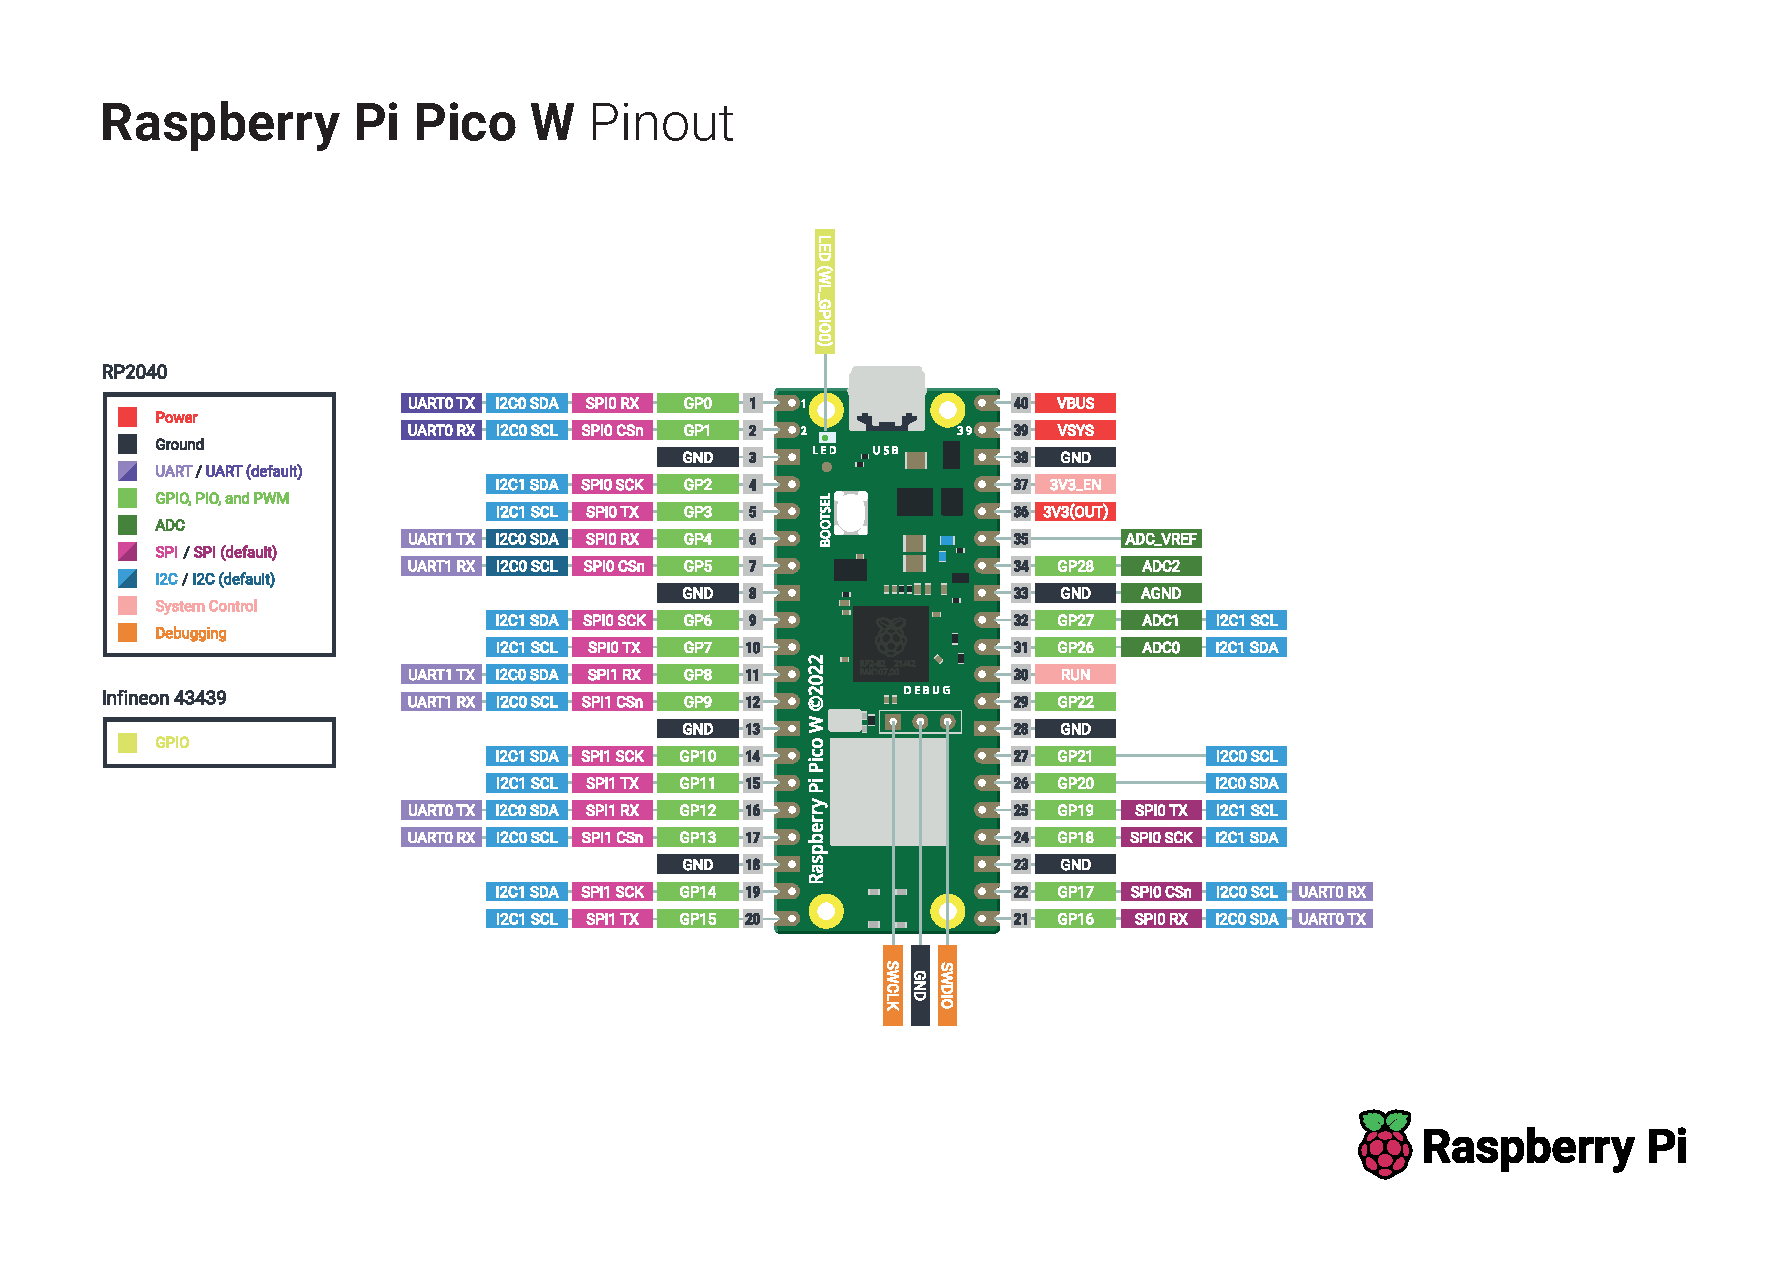
\includegraphics[width=\linewidth]{Introduccion/img/raspberry-pi-pico-w-pinout}
	\caption{Raspberry Pi Pico W Pinout.}
	\label{fig:raspberry-pi-pico-w-pinout}
\end{figure}

Como sabemos dentro del mercado de los microcontroladores existen una gran variedad de ellos. \textcolor{blue}{¿Porqué entonces elegimos este en particular?} El RP2040 posee un periférico en particular denominado PIO (Programable Input/Output), podríamos pensar a dicho periférico como un fragmento de FPGA en su idea central, dado que ambos te permiten crear un hardware a medida que se adapta a señales digitales que con periféricos existentes no es posible. La diferencia es que con una FPGA se define una lógica (por ejemplo utilizando flip-flops, FSMs, Sumadores, etc) y diciendo como estos deben conectarse. Con el PIO se programan unas máquinas de estados que ejecutan un conjunto de instrucciones para leer/generar señales de forma determinista y concurrente. Este microcontrolador posee un conjunto de 8 máquinas de estado. Al estar embebido dentro del propio microcontrolador permite manipularlo junto con otros periféricos dentro del mismo. En particular permite controlar los propios GPIOs. Entonces la idea detrás del Generador de Funciones consiste en producir un DAC (conversor de digital a analógico) que pueda actuar a altas velocidades. El proceso sería primero tener cargado en RAM cada punto de la señal a muestrear, luego transferirlo mediante DMA hacia el periférico PIO y que este mismo se encargue de producir el valor de tensión deseado habilitando o no salidas GPIOs mediante un DAC R2R (el cual puede verse en la figura ).

\begin{figure}[H]
	\centering
	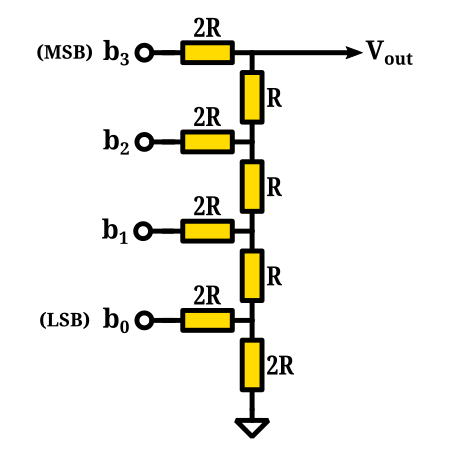
\includegraphics[width=0.5\linewidth]{Introduccion/img/r2r-4bits-2}
	\caption{DAC R-2R de 4 Bits. Este tipo de DAC permite tener un valor de tensión de acuerdo a la cantidad de bits habilitados y su ponderación. La resolución (mínima representación de valor de tensión) depende de la cantidad de bits. Con 4 bits y una alimentación de 3V3 la resolución es de 206 mV.}
	\label{fig:r2r-4bits-2}
\end{figure}

Este proyecto consiste en la continuación de un trabajo que se realizó en otras materias. Este proyecto base es el generador de funciones arbitrarias con dicho micro realizado con el conjunto de resistencias R-2R. La idea sería poder realizar un dispositivo completo con una mejora clara a nivel tecnológico. Partiendo de que la base de usar un DAC con resistencias R-2R se cambiarían por un sintetizador digital directo (DDS). En particular se quiere utilizar el AD9102 que tiene 12 bits de resolución a comparación de los 8 bits implementados en la versión anterior. También hay cierta mejoras respecto a la corriente máxima que permite a la salida del conector BNC, así como la impedancia de salida que sea de $50 \ \Omega$. Las versiones anteriores no dejaban de ser prototipos, la idea ahora es realizar un equipo completo en donde se tengan las placas de desarrollos diseñadas, una fuente de alimentación conmutada conectada a 220 Vac y una carcasa en 3D o en su caso en chapa.

\section{Motivación}
La motivación para realizar el proyecto comenzó como parte de un trabajo práctico de la materia \textit{Dispositivos y Circuitos Electrónicos IV} donde se realizó una primera versión del desarrollo. El trabajo únicamente consistía en generar la señal con el DAC 2-2R y eligiendo mediante una pantalla TFT el valor de la frecuencia de salida. Debido al tiempo limitado el hardware se realizó lo mencionado, quedando como futura mejora la implementación de un control de acondicionamiento de señal, permitiendo variar el amplitud máxima, offset y tipo de señal. Por el lado del firmware de la primera versión un Framework que permite modelar máquinas de estados jerárquicas. Este Framework se llama \textbf{Quantum Leaps}. A continuación se muestra una foto de la primera versión realizada en una placa perforada y luego la MEF implementada.

\begin{figure}[H]
	\centering
	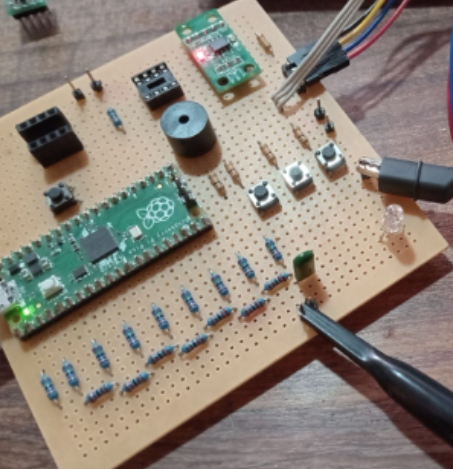
\includegraphics[width=0.5\linewidth]{Introduccion/img/1raVersionPlaca}
	\caption{Primera versión de la placa de desarrollo, realizada con una placa perforada.}
	\label{fig:1raversionplaca}
\end{figure}

\begin{figure}[H]
	\centering
	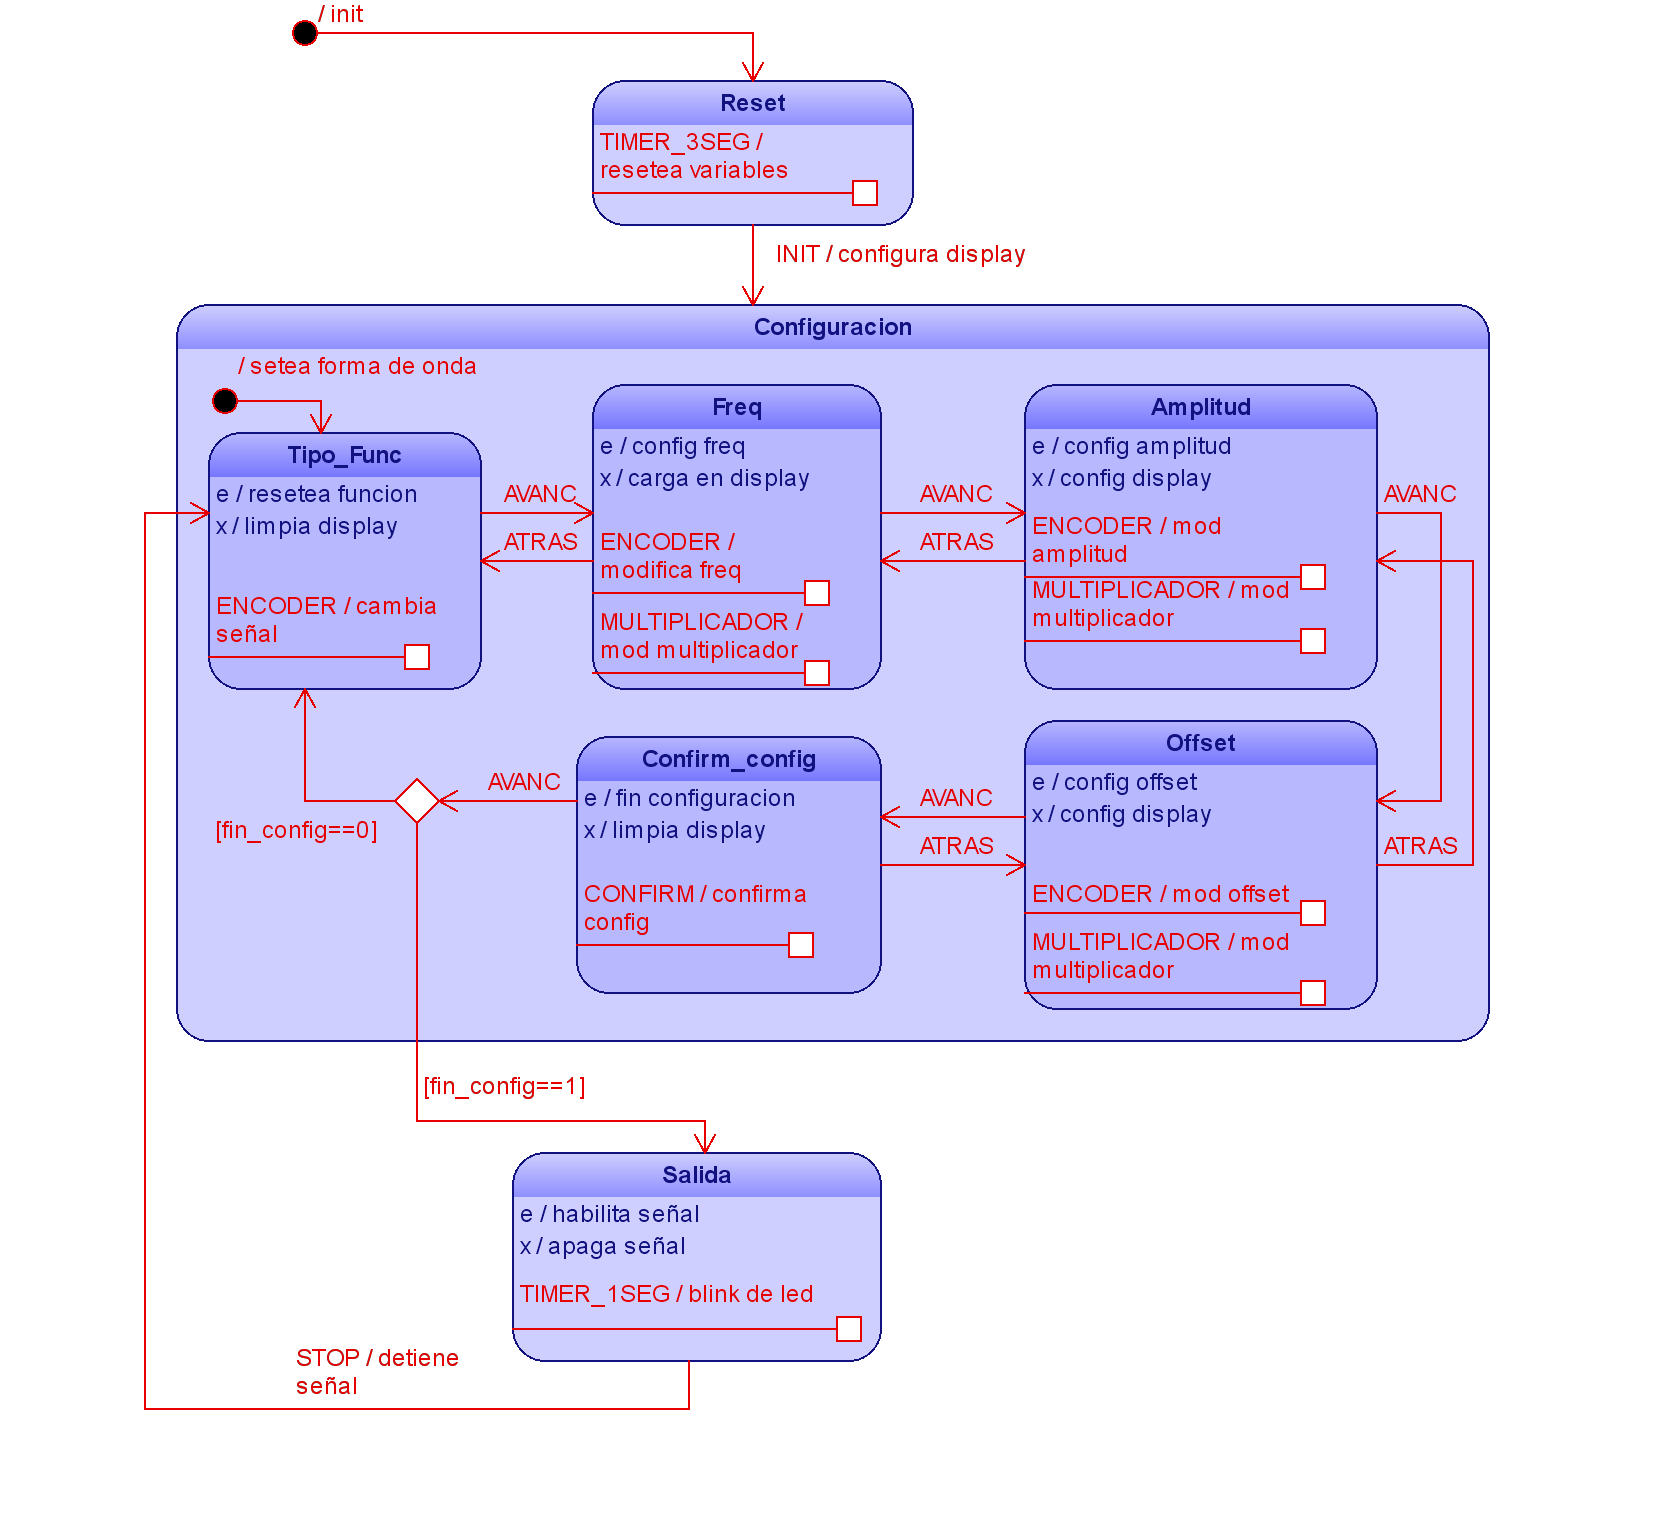
\includegraphics[width=0.7\linewidth]{Introduccion/img/SM_of_Awg}
	\caption{Máquina de estado implementada en el modelado.}
	\label{fig:smofawg}
\end{figure}

A grandes rasgos se pueden observar tres estados principales (\textbf{Reset},\textbf{Configuración} y \textbf{Salida}). Luego dentro de \textit{Configuración} se tienen sus respectivos sub-estados. La idea detrás de esta MEF es permitir que el usuario permita una configuración de cada parámetro del generado de funciones realizado observando los cambios en una pantalla TFT de 2.4 in. Tal como se mencionó solamente permitía configurarse la frecuencia en la primera versión del proyecto, por lo que los sub-estados \textit{Amplitud, Offset} estaban deshabilitados.

Posteriormente dicho proyecto fue continuado en la materia de \textit{Sistemas Embebidos Avanzados II}. Uno de los contenidos de dicha materia es programación en \textit{Sistemas Operativos en Tiempo Real} ()\textbf{RTOS}). En particular se utilizó el conocido \textbf{FreeRTOS}. Como trabajo final para la materia se decidió continuar con el proyecto ya mencionado, agregándole en este caso el \textbf{FreeRTOS} junto con la máquina de estado que ya formaba parte del proyecto base. Como mejora a nivel de Hardware se procedió a realizar una PCB de doble capa, la cual se mandó a realizar a China en \textbf{JLCPCB}. Se puede visualizar a continuación una imagen de dicha PCB.

\begin{figure}[H]
	\centering
	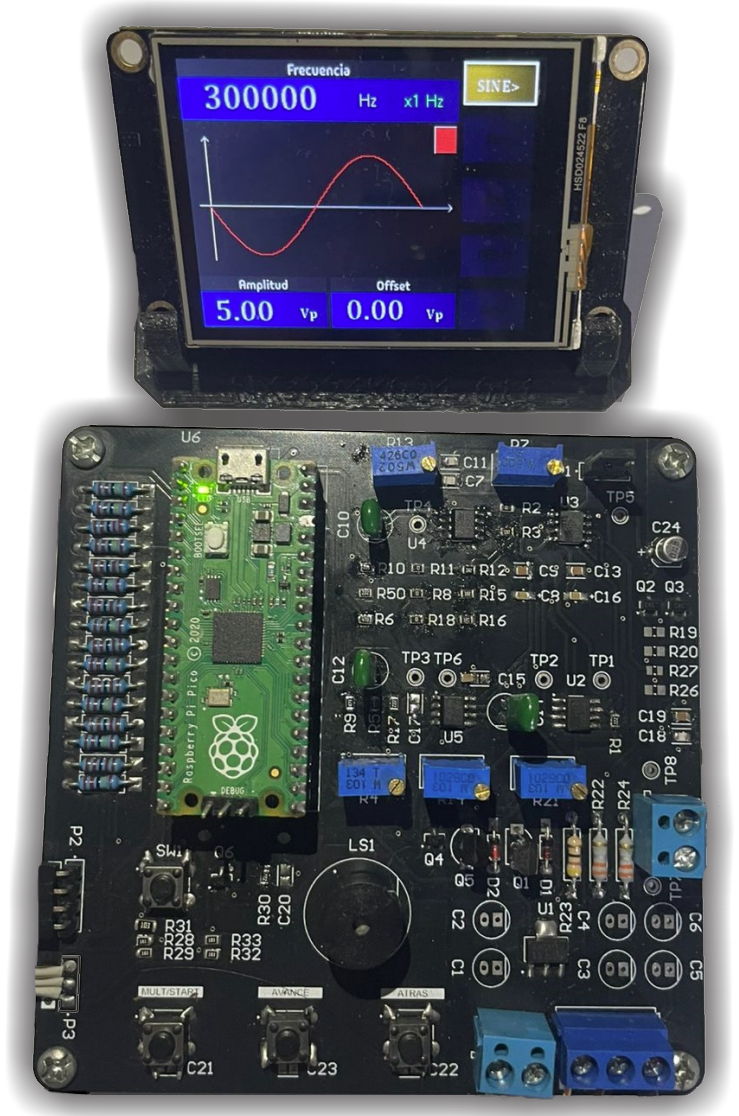
\includegraphics[width=0.6\linewidth]{Introduccion/img/dispositivo}
	\caption{Segunda versión de la PCB del generador de funciones Arbitrario.}
	\label{fig:dispositivo}
\end{figure}

En esta versión ya se puede ver claramente las distintas partes que componen el circuito en la capa Top. Por un lado se tiene el DAC R-2R junto con el micro. Por el lado derecho se tiene la lógica de control. Dentro de estas mejoras de Hardware ya se incluyó la posibilidad de generar una amplificación de la señal, junto con el offset respectivo. Para poder realizar esto se utilizó un potenciómetro digital, señales PWM (junto con filtros \textit{Pasa Bajos Activos}) y operacionales. Dado que dentro de las características solicitadas se había la mencionado la posibilidad de poder generar señales de hasta 1 MHz, aparecía una limitación en la ganancia máxima a dicha frecuencia y en el Slew Rate máximo en el promedio de los Operacionales que se venden en el mercado local. De esta forma se procedió a una investigación sobre los Amplificadores Operacionales disponibles en Mercado Libre que permitieran tener una Ganancia considerable a alta frecuencia y además un elevado Slew Rate. Luego de este proceso se optó por el LM6172 que tiene un ancho de banda de 100 MHz y un Slew Rate 3000 V/$\mu$S.

Para poder visualizar la información que el usuario va configurando se utilizó una pantalla TFT Nextion de 2.4 in. Para esto posee un enconder rotativo de 20 vueltas (no se observa en la imagen) y pulsadores para avanzar, retroceder y cambiar el multiplicador (de tensión, frecuencia y offset). Una vez que el usuario termina de configurar la salida luego esta señal se carga en un buffer y se procede a muestrear a través de los periféricos \textbf{DMA} y \textbf{PIO}. En particular se muestra un ejemplo de una salida senoidal con 10 Vpp y 50 KHz.

\begin{figure}[H]
	\centering
	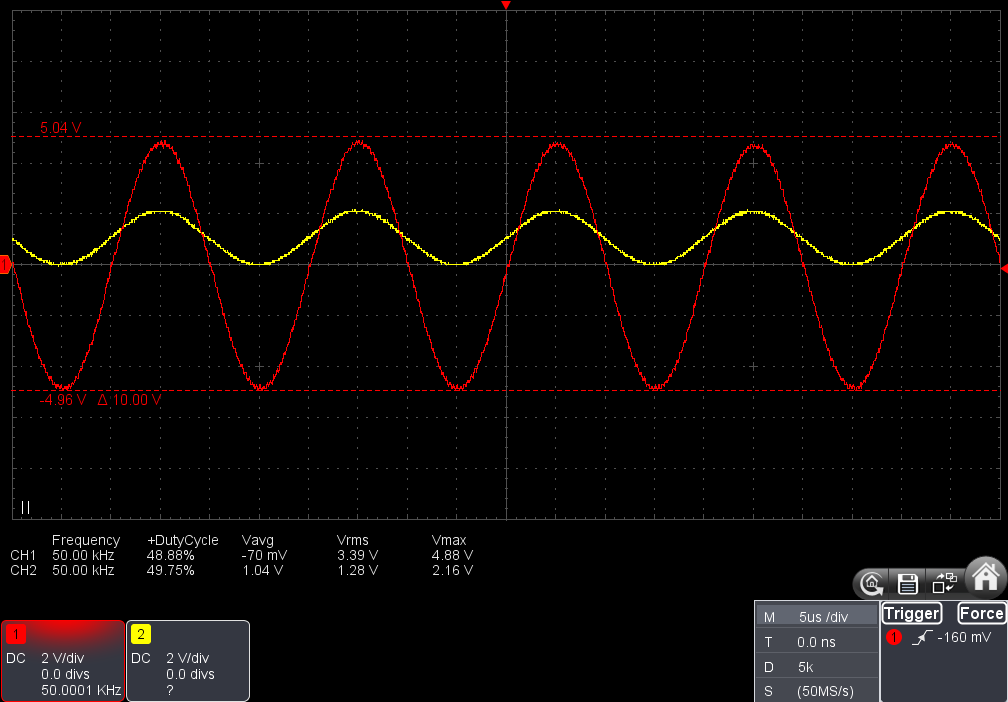
\includegraphics[width=0.7\linewidth]{Introduccion/img/10VPP_50KHZ_SENOIDAL}
	\caption{Señal Senoidal con una amplitud de 10 Vpp y 50 KHz.}
	\label{fig:10vpp50khzsenoidal}
\end{figure}

En amarillo se puede observar la señal que sale desde el DAC R-2R y en rojo la señal amplificada y con offset nulo.